
%% bare_jrnl.tex
%% V1.3
%% 2007/01/11
%% by Michael Shell
%% see http://www.michaelshell.org/
%% for current contact information.
%%
%% This is a skeleton file demonstrating the use of IEEEtran.cls
%% (requires IEEEtran.cls version 1.7 or later) with an IEEE journal paper.
%%
%% Support sites:
%% http://www.michaelshell.org/tex/ieeetran/
%% http://www.ctan.org/tex-archive/macros/latex/contrib/IEEEtran/
%% and
%% http://www.ieee.org/



% *** Authors should verify (and, if needed, correct) their LaTeX system  ***
% *** with the testflow diagnostic prior to trusting their LaTeX platform ***
% *** with production work. IEEE's font choices can trigger bugs that do  ***
% *** not appear when using other class files.                            ***
% The testflow support page is at:
% http://www.michaelshell.org/tex/testflow/


%%*************************************************************************
%% Legal Notice:
%% This code is offered as-is without any warranty either expressed or
%% implied; without even the implied warranty of MERCHANTABILITY or
%% FITNESS FOR A PARTICULAR PURPOSE!
%% User assumes all risk.
%% In no event shall IEEE or any contributor to this code be liable for
%% any damages or losses, including, but not limited to, incidental,
%% consequential, or any other damages, resulting from the use or misuse
%% of any information contained here.
%%
%% All comments are the opinions of their respective authors and are not
%% necessarily endorsed by the IEEE.
%%
%% This work is distributed under the LaTeX Project Public License (LPPL)
%% ( http://www.latex-project.org/ ) version 1.3, and may be freely used,
%% distributed and modified. A copy of the LPPL, version 1.3, is included
%% in the base LaTeX documentation of all distributions of LaTeX released
%% 2003/12/01 or later.
%% Retain all contribution notices and credits.
%% ** Modified files should be clearly indicated as such, including  **
%% ** renaming them and changing author support contact information. **
%%
%% File list of work: IEEEtran.cls, IEEEtran_HOWTO.pdf, bare_adv.tex,
%%                    bare_conf.tex, bare_jrnl.tex, bare_jrnl_compsoc.tex
%%*************************************************************************

% Note that the a4paper option is mainly intended so that authors in
% countries using A4 can easily print to A4 and see how their papers will
% look in print - the typesetting of the document will not typically be
% affected with changes in paper size (but the bottom and side margins will).
% Use the testflow package mentioned above to verify correct handling of
% both paper sizes by the user's LaTeX system.
%
% Also note that the "draftcls" or "draftclsnofoot", not "draft", option
% should be used if it is desired that the figures are to be displayed in
% draft mode.
%
\documentclass[journal]{IEEEtran}
%
% If IEEEtran.cls has not been installed into the LaTeX system files,
% manually specify the path to it like:
% \documentclass[journal]{../sty/IEEEtran}





% Some very useful LaTeX packages include:
% (uncomment the ones you want to load)


% *** MISC UTILITY PACKAGES ***
%
%\usepackage{ifpdf}
% Heiko Oberdiek's ifpdf.sty is very useful if you need conditional
% compilation based on whether the output is pdf or dvi.
% usage:
% \ifpdf
%   % pdf code
% \else
%   % dvi code
% \fi
% The latest version of ifpdf.sty can be obtained from:
% http://www.ctan.org/tex-archive/macros/latex/contrib/oberdiek/
% Also, note that IEEEtran.cls V1.7 and later provides a builtin
% \ifCLASSINFOpdf conditional that works the same way.
% When switching from latex to pdflatex and vice-versa, the compiler may
% have to be run twice to clear warning/error messages.






% *** CITATION PACKAGES ***
%
\usepackage{cite}
% cite.sty was written by Donald Arseneau
% V1.6 and later of IEEEtran pre-defines the format of the cite.sty package
% \cite{} output to follow that of IEEE. Loading the cite package will
% result in citation numbers being automatically sorted and properly
% "compressed/ranged". e.g., [1], [9], [2], [7], [5], [6] without using
% cite.sty will become [1], [2], [5]--[7], [9] using cite.sty. cite.sty's
% \cite will automatically add leading space, if needed. Use cite.sty's
% noadjust option (cite.sty V3.8 and later) if you want to turn this off.
% cite.sty is already installed on most LaTeX systems. Be sure and use
% version 4.0 (2003-05-27) and later if using hyperref.sty. cite.sty does
% not currently provide for hyperlinked citations.
% The latest version can be obtained at:
% http://www.ctan.org/tex-archive/macros/latex/contrib/cite/
% The documentation is contained in the cite.sty file itself.






% *** GRAPHICS RELATED PACKAGES ***
%
\ifCLASSINFOpdf
  \usepackage[pdftex]{graphicx}
  % declare the path(s) where your graphic files are
  % \graphicspath{{../pdf/}{../jpeg/}}
  % and their extensions so you won't have to specify these with
  % every instance of \includegraphics
  % \DeclareGraphicsExtensions{.pdf,.jpeg,.png}
\else
  % or other class option (dvipsone, dvipdf, if not using dvips). graphicx
  % will default to the driver specified in the system graphics.cfg if no
  % driver is specified.
  % \usepackage[dvips]{graphicx}
  % declare the path(s) where your graphic files are
  % \graphicspath{{../eps/}}
  % and their extensions so you won't have to specify these with
  % every instance of \includegraphics
  % \DeclareGraphicsExtensions{.eps}
\fi
% graphicx was written by David Carlisle and Sebastian Rahtz. It is
% required if you want graphics, photos, etc. graphicx.sty is already
% installed on most LaTeX systems. The latest version and documentation can
% be obtained at:
% http://www.ctan.org/tex-archive/macros/latex/required/graphics/
% Another good source of documentation is "Using Imported Graphics in
% LaTeX2e" by Keith Reckdahl which can be found as epslatex.ps or
% epslatex.pdf at: http://www.ctan.org/tex-archive/info/
%
% latex, and pdflatex in dvi mode, support graphics in encapsulated
% postscript (.eps) format. pdflatex in pdf mode supports graphics
% in .pdf, .jpeg, .png and .mps (metapost) formats. Users should ensure
% that all non-photo figures use a vector format (.eps, .pdf, .mps) and
% not a bitmapped formats (.jpeg, .png). IEEE frowns on bitmapped formats
% which can result in "jaggedy"/blurry rendering of lines and letters as
% well as large increases in file sizes.
%
% You can find documentation about the pdfTeX application at:
% http://www.tug.org/applications/pdftex





% *** MATH PACKAGES ***
%
%\usepackage[cmex10]{amsmath}
% A popular package from the American Mathematical Society that provides
% many useful and powerful commands for dealing with mathematics. If using
% it, be sure to load this package with the cmex10 option to ensure that
% only type 1 fonts will utilized at all point sizes. Without this option,
% it is possible that some math symbols, particularly those within
% footnotes, will be rendered in bitmap form which will result in a
% document that can not be IEEE Xplore compliant!
%
% Also, note that the amsmath package sets \interdisplaylinepenalty to 10000
% thus preventing page breaks from occurring within multiline equations. Use:
%\interdisplaylinepenalty=2500
% after loading amsmath to restore such page breaks as IEEEtran.cls normally
% does. amsmath.sty is already installed on most LaTeX systems. The latest
% version and documentation can be obtained at:
% http://www.ctan.org/tex-archive/macros/latex/required/amslatex/math/





% *** SPECIALIZED LIST PACKAGES ***
%
\usepackage{algorithmic}
% algorithmic.sty was written by Peter Williams and Rogerio Brito.
% This package provides an algorithmic environment fo describing algorithms.
% You can use the algorithmic environment in-text or within a figure
% environment to provide for a floating algorithm. Do NOT use the algorithm
% floating environment provided by algorithm.sty (by the same authors) or
% algorithm2e.sty (by Christophe Fiorio) as IEEE does not use dedicated
% algorithm float types and packages that provide these will not provide
% correct IEEE style captions. The latest version and documentation of
% algorithmic.sty can be obtained at:
% http://www.ctan.org/tex-archive/macros/latex/contrib/algorithms/
% There is also a support site at:
% http://algorithms.berlios.de/index.html
% Also of interest may be the (relatively newer and more customizable)
% algorithmicx.sty package by Szasz Janos:
% http://www.ctan.org/tex-archive/macros/latex/contrib/algorithmicx/




% *** ALIGNMENT PACKAGES ***
%
%\usepackage{array}
% Frank Mittelbach's and David Carlisle's array.sty patches and improves
% the standard LaTeX2e array and tabular environments to provide better
% appearance and additional user controls. As the default LaTeX2e table
% generation code is lacking to the point of almost being broken with
% respect to the quality of the end results, all users are strongly
% advised to use an enhanced (at the very least that provided by array.sty)
% set of table tools. array.sty is already installed on most systems. The
% latest version and documentation can be obtained at:
% http://www.ctan.org/tex-archive/macros/latex/required/tools/


%\usepackage{mdwmath}
%\usepackage{mdwtab}
% Also highly recommended is Mark Wooding's extremely powerful MDW tools,
% especially mdwmath.sty and mdwtab.sty which are used to format equations
% and tables, respectively. The MDWtools set is already installed on most
% LaTeX systems. The lastest version and documentation is available at:
% http://www.ctan.org/tex-archive/macros/latex/contrib/mdwtools/


% IEEEtran contains the IEEEeqnarray family of commands that can be used to
% generate multiline equations as well as matrices, tables, etc., of high
% quality.


%\usepackage{eqparbox}
% Also of notable interest is Scott Pakin's eqparbox package for creating
% (automatically sized) equal width boxes - aka "natural width parboxes".
% Available at:
% http://www.ctan.org/tex-archive/macros/latex/contrib/eqparbox/




% *** SUBFIGURE PACKAGES ***
\usepackage[tight,footnotesize]{subfigure}
% subfigure.sty was written by Steven Douglas Cochran. This package makes it
% easy to put subfigures in your figures. e.g., "Figure 1a and 1b". For IEEE
% work, it is a good idea to load it with the tight package option to reduce
% the amount of white space around the subfigures. subfigure.sty is already
% installed on most LaTeX systems. The latest version and documentation can
% be obtained at:
% http://www.ctan.org/tex-archive/obsolete/macros/latex/contrib/subfigure/
% subfigure.sty has been superceeded by subfig.sty.



%\usepackage[caption=false]{caption}
%\usepackage[font=footnotesize]{subfig}
% subfig.sty, also written by Steven Douglas Cochran, is the modern
% replacement for subfigure.sty. However, subfig.sty requires and
% automatically loads Axel Sommerfeldt's caption.sty which will override
% IEEEtran.cls handling of captions and this will result in nonIEEE style
% figure/table captions. To prevent this problem, be sure and preload
% caption.sty with its "caption=false" package option. This is will preserve
% IEEEtran.cls handing of captions. Version 1.3 (2005/06/28) and later
% (recommended due to many improvements over 1.2) of subfig.sty supports
% the caption=false option directly:
%\usepackage[caption=false,font=footnotesize]{subfig}
%
% The latest version and documentation can be obtained at:
% http://www.ctan.org/tex-archive/macros/latex/contrib/subfig/
% The latest version and documentation of caption.sty can be obtained at:
% http://www.ctan.org/tex-archive/macros/latex/contrib/caption/




% *** FLOAT PACKAGES ***
%
%\usepackage{fixltx2e}
% fixltx2e, the successor to the earlier fix2col.sty, was written by
% Frank Mittelbach and David Carlisle. This package corrects a few problems
% in the LaTeX2e kernel, the most notable of which is that in current
% LaTeX2e releases, the ordering of single and double column floats is not
% guaranteed to be preserved. Thus, an unpatched LaTeX2e can allow a
% single column figure to be placed prior to an earlier double column
% figure. The latest version and documentation can be found at:
% http://www.ctan.org/tex-archive/macros/latex/base/



\usepackage{stfloats}
% stfloats.sty was written by Sigitas Tolusis. This package gives LaTeX2e
% the ability to do double column floats at the bottom of the page as well
% as the top. (e.g., "\begin{figure*}[!b]" is not normally possible in
% LaTeX2e). It also provides a command:
%\fnbelowfloat
% to enable the placement of footnotes below bottom floats (the standard
% LaTeX2e kernel puts them above bottom floats). This is an invasive package
% which rewrites many portions of the LaTeX2e float routines. It may not work
% with other packages that modify the LaTeX2e float routines. The latest
% version and documentation can be obtained at:
% http://www.ctan.org/tex-archive/macros/latex/contrib/sttools/
% Documentation is contained in the stfloats.sty comments as well as in the
% presfull.pdf file. Do not use the stfloats baselinefloat ability as IEEE
% does not allow \baselineskip to stretch. Authors submitting work to the
% IEEE should note that IEEE rarely uses double column equations and
% that authors should try to avoid such use. Do not be tempted to use the
% cuted.sty or midfloat.sty packages (also by Sigitas Tolusis) as IEEE does
% not format its papers in such ways.


\ifCLASSOPTIONcaptionsoff
  \usepackage[nomarkers]{endfloat}
 \let\MYoriglatexcaption\caption
 \renewcommand{\caption}[2][\relax]{\MYoriglatexcaption[#2]{#2}}
\fi
% endfloat.sty was written by James Darrell McCauley and Jeff Goldberg.
% This package may be useful when used in conjunction with IEEEtran.cls'
% captionsoff option. Some IEEE journals/societies require that submissions
% have lists of figures/tables at the end of the paper and that
% figures/tables without any captions are placed on a page by themselves at
% the end of the document. If needed, the draftcls IEEEtran class option or
% \CLASSINPUTbaselinestretch interface can be used to increase the line
% spacing as well. Be sure and use the nomarkers option of endfloat to
% prevent endfloat from "marking" where the figures would have been placed
% in the text. The two hack lines of code above are a slight modification of
% that suggested by in the endfloat docs (section 8.3.1) to ensure that
% the full captions always appear in the list of figures/tables - even if
% the user used the short optional argument of \caption[]{}.
% IEEE papers do not typically make use of \caption[]'s optional argument,
% so this should not be an issue. A similar trick can be used to disable
% captions of packages such as subfig.sty that lack options to turn off
% the subcaptions:
% For subfig.sty:
% \let\MYorigsubfloat\subfloat
% \renewcommand{\subfloat}[2][\relax]{\MYorigsubfloat[]{#2}}
% For subfigure.sty:
% \let\MYorigsubfigure\subfigure
% \renewcommand{\subfigure}[2][\relax]{\MYorigsubfigure[]{#2}}
% However, the above trick will not work if both optional arguments of
% the \subfloat/subfig command are used. Furthermore, there needs to be a
% description of each subfigure *somewhere* and endfloat does not add
% subfigure captions to its list of figures. Thus, the best approach is to
% avoid the use of subfigure captions (many IEEE journals avoid them anyway)
% and instead reference/explain all the subfigures within the main caption.
% The latest version of endfloat.sty and its documentation can obtained at:
% http://www.ctan.org/tex-archive/macros/latex/contrib/endfloat/
%
% The IEEEtran \ifCLASSOPTIONcaptionsoff conditional can also be used
% later in the document, say, to conditionally put the References on a
% page by themselves.





% *** PDF, URL AND HYPERLINK PACKAGES ***
%
\usepackage{url}
% url.sty was written by Donald Arseneau. It provides better support for
% handling and breaking URLs. url.sty is already installed on most LaTeX
% systems. The latest version can be obtained at:
% http://www.ctan.org/tex-archive/macros/latex/contrib/misc/
% Read the url.sty source comments for usage information. Basically,
% \url{my_url_here}.





% *** Do not adjust lengths that control margins, column widths, etc. ***
% *** Do not use packages that alter fonts (such as pslatex).         ***
% There should be no need to do such things with IEEEtran.cls V1.6 and later.
% (Unless specifically asked to do so by the journal or conference you plan
% to submit to, of course. )


% correct bad hyphenation here
\hyphenation{op-tical net-works semi-conduc-tor}



\begin{document}
%
% paper title
% can use linebreaks \\ within to get better formatting as desired
\title{Dynamical Handling of Straddle Carriers Activities on a Container
Terminal in Uncertain Environment \\ \textit{- A Swarm Intelligence approach -}}
%
%
% author names and IEEE memberships
% note positions of commas and nonbreaking spaces ( ~ ) LaTeX will not break
% a structure at a ~ so this keeps an author's name from being broken across
% two lines.
% use \thanks{} to gain access to the first footnote area
% a separate \thanks must be used for each paragraph as LaTeX2e's \thanks
% was not built to handle multiple paragraphs
%

\author{
Stefan~Balev, Fr\'{e}d\'{e}ric~Guinand,
Ga\"{e}tan~Lesauvage$^*$\thanks{$^*$~Corresponding author.}, Damien~Olivier\\
\medskip
Universit\'{e} du Havre, LITIS EA 4108\\
BP 540, 76058 Le Havre, France\\
\medskip
E-mail:
\texttt{\{stefan.balev,frederic.guinand,damien.olivier\}@univ-lehavre.fr,
gaetanlesauvage@gmail.com}
}

% note the % following the last \IEEEmembership and also \thanks -
% these prevent an unwanted space from occurring between the last author name
% and the end of the author line. i.e., if you had this:
%
% \author{....lastname \thanks{...} \thanks{...} }
%                     ^------------^------------^----Do not want these spaces!
%
% a space would be appended to the last name and could cause every name on that
% line to be shifted left slightly. This is one of those "LaTeX things". For
% instance, "\textbf{A} \textbf{B}" will typeset as "A B" not "AB". To get
% "AB" then you have to do: "\textbf{A}\textbf{B}"
% \thanks is no different in this regard, so shield the last } of each \thanks
% that ends a line with a % and do not let a space in before the next \thanks.
% Spaces after \IEEEmembership other than the last one are OK (and needed) as
% you are supposed to have spaces between the names. For what it is worth,
% this is a minor point as most people would not even notice if the said evil
% space somehow managed to creep in.



% The paper headers
%\markboth{Journal of \LaTeX\ Class Files,~Vol.~6, No.~1, January~2007}%
%{Shell \MakeLowercase{\textit{et al.}}: Bare Demo of IEEEtran.cls for Journals}
% The only time the second header will appear is for the odd numbered pages
% after the title page when using the twoside option.
%
% *** Note that you probably will NOT want to include the author's ***
% *** name in the headers of peer review papers.                   ***
% You can use \ifCLASSOPTIONpeerreview for conditional compilation here if
% you desire.




% If you want to put a publisher's ID mark on the page you can do it like
% this:
%\IEEEpubid{0000--0000/00\$00.00~\copyright~2007 IEEE}
% Remember, if you use this you must call \IEEEpubidadjcol in the second
% column for its text to clear the IEEEpubid mark.



% use for special paper notices
%\IEEEspecialpapernotice{(Invited Paper)}




% make the title area
\maketitle


\begin{abstract}
%\boldmath
    The CALAS project consists in a laser measure system allowing to localize precisely straddle carriers in a container terminal. The information given by such a tool makes an optimization possible. In fact, a box terminal is an open system subject to dynamics, in which many events can occur. Among others, they concern
container arrivals and departures. Within the terminal, straddle carriers are trucks which are able to carry one container at a time in order to move it through the terminal. We aim to optimize the straddle carrier handling in order to improve the terminal management. Moreover, missions come into the system in an
unpredictable way and straddle carriers are handled by humans. They can choose to follow the schedule or not. For these reasons, the exact state of the system is unknown. The optimization process that we try to build must be fail-safe and adaptive. In this context, we propose an approach using a meta-heuristic based on Ant Colony to resolve the problem of assigning missions to straddle carriers. We built a simulator which is able to test and to compare different scheduling policies.
\\
\end{abstract}
% IEEEtran.cls defaults to using nonbold math in the Abstract.
% This preserves the distinction between vectors and scalars. However,
% if the journal you are submitting to favors bold math in the abstract,
% then you can use LaTeX's standard command \boldmath at the very start
% of the abstract to achieve this. Many IEEE journals frown on math
% in the abstract anyway.

% Note that keywords are not normally used for peerreview papers.
\begin{IEEEkeywords}
 swarm intelligence, colored ant colony system, dynamic graph, multiple criteria
optimization, vehicle routing problem, container terminal.
\end{IEEEkeywords}

\section{System description}

%\subsection{The CALAS project}

The CALAS project aims at localizing precisely handling trucks on a box
terminal. It uses a laser localizing system and software which allows to deal
with the data sent by laser sensors. This project is the result of a collaboration
between \textit{Laser Data Technology Terminal} company and the
\textit{Terminaux de Normandie} company. The goal of the CALAS project is to
know the state of the terminal in real time, meaning both containers and
vehicles location.

%\subsection{Container terminal}

A container terminal is divided into three main areas (see Fig. \ref{terminalDeNormandie}). Each part is a set of
box rows where containers can be stacked up and these areas are linked by
oriented roads. The first area is the quayside. It is beside a channel where
ships can tie to the dockside. It is an area bound to prepare the ship
(un)loading. The second area, the landside, is used to load or unload trucks
and trains. The third part is a storing area linking the two others. Containers
are moved into this area when a ship, a truck or a train is unloaded, and
containers are moved from this area when a ship, a truck or a train is loaded.
Managing a box terminal involves three kinds of tasks:

\begin{itemize}
	\item Preparing a ship (un)loading;
	\item Preparing a truck (or a train) (un)loading;
	\item Optimizing storing area.
\end{itemize}

In order to accomplish these tasks, containers are moved from one
position to another. Such moves are called missions. Each mission is
assigned to a straddle carrier.

\begin{figure}[h]
\fbox{\begin{minipage}{0.475\textwidth}
	\begin{center}
	
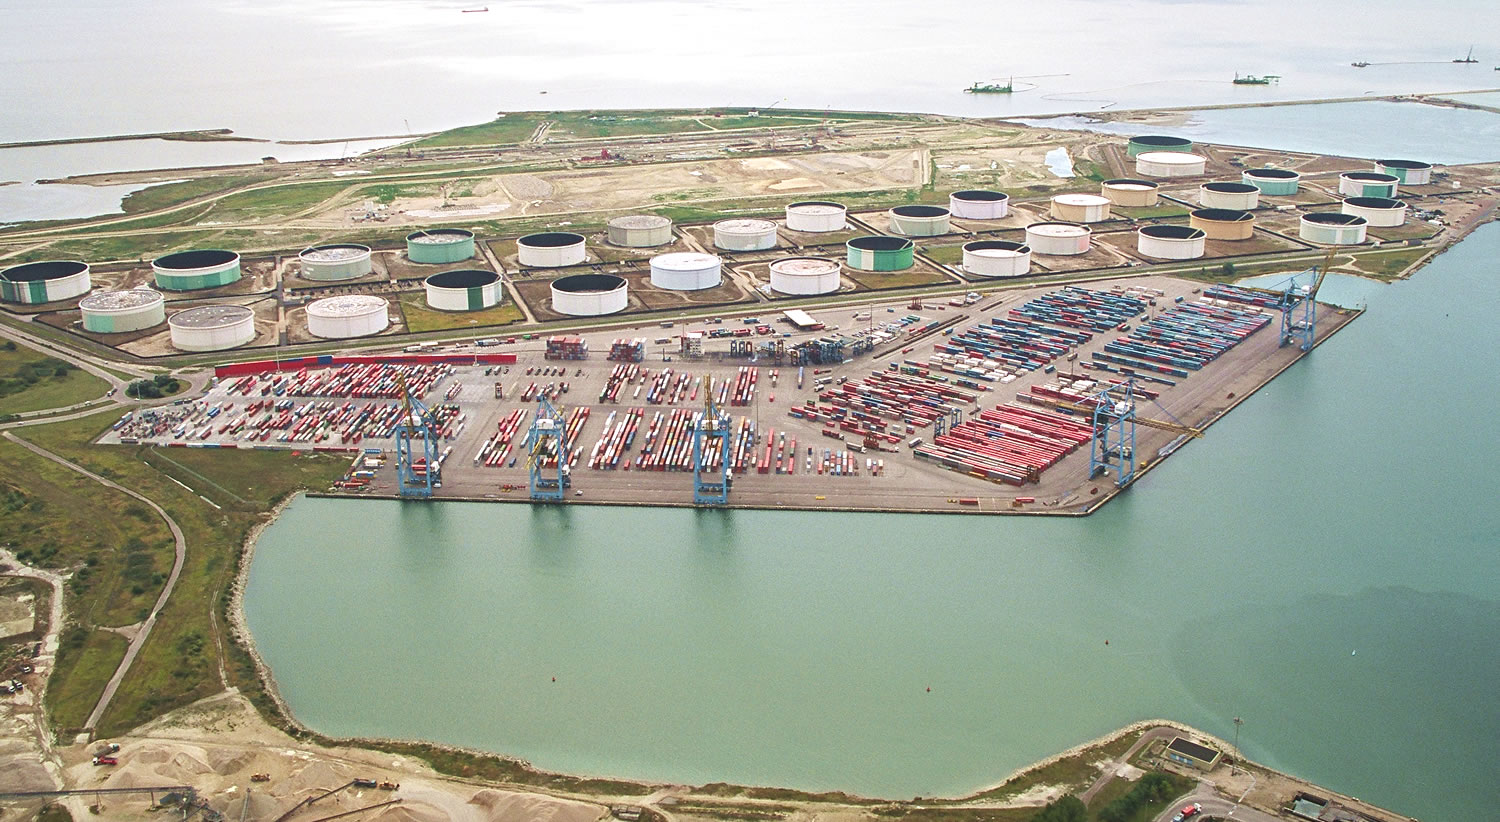
\includegraphics[width=\textwidth]{Shemas/terminalDeNormandie.jpg} \\
	\end{center}
\end{minipage}}
\caption[Terminal de Normandie, Le Havre, France]{Terminal de Normandie, Le
Havre, France\protect \footnotemark.}
\label{terminalDeNormandie}
\end{figure}
\footnotetext{source: http://www.t-n.fr/tn.htm}

The container terminal is an open system subject to dynamics. Though a
subset of missions is known before starting the schedule, new missions arise when the schedule has already been established and its execution has started. Moreover, trucks
arriving time is not known precisely enough to forecast container delivery. If a truck is late, the straddle carrier which has to load or unload it, could be assigned to another mission instead of staying idle
and waiting for the truck. Human behavior also affects the system because straddle carriers are handled by human drivers who can choose to follow the schedule or not.


\section{Related Work}
%State of the art of current optimization
In such a system, the turn around time of both vessels and trucks/trains has to
be as small as possible. Three different ways have already been used to solve
this real problem.

%1. Analytical
 First, the analytical approach is based on a study of interrelated factors
which have to be taken into account to improve the efficiency of the system. In \cite{murty2005}, an integrative decision support system is described. It has been created by studying inter-related decisions made daily in a container terminal. The authors evaluated the system at a terminal in Hong Kong and measured a reduction of 30\% of the ships turn around time and the costs of container handling have dropped by 35\%.

%2. Simulation
The second approach is the simulation. It consists in building a simulator which
is able to test several methods of optimization. In \cite{jin2004}, the authors have used both a genetic algorithm and a neural network system for the regulation of container yard operations. With 2 berths, 64
blocks, a planning period of 24h and a forecast period of 3 days, their simulation had shown a reduction of the total ship waiting time from 64h to 46h.
In \cite{ottjes2006}, the authors tried to improve the performance of the Rotterdam's Maasvlakte port area in studying its design. Their simulation gives information about quay length, storage capacity and
handling and transport equipment of the terminal. Their results are useful for
designing the next terminals.

%3. Multi Agent
The last approach is the multi-agent system (MAS). Thurston and Hu \cite{thurston2002} aimed at improving the performance of the terminal by a dynamic and cooperative rescheduling of quay cranes and straddle carriers. Here
each part of the system is considered as an autonomous agent able to take decisions according to the information of its own environment. Henesey \textit{et al.} \cite{Henesey2002-1,Henesey2002-2,Henesey2003,Henesey2004}
have developed this idea. Their agents try to reach their own goal by searching, coordinating, communicating, and negotiating with other agents. They take their decisions according to a market based mechanism. Like in an
auction, they bid for winning a task. Their system allows to test several policies of berthing, stacking or sequencing. They figured out that good decisions about stacking and berth allocation impact positively on the vessel turn around time.

%Transition
According to these last conclusions, it appears that optimizing the performance
of a container terminal means handling the vehicles' moves and their missions
allocation. In this context, we deal with a vehicle routing problem.

\section{Vehicle Routing Problems}
 
Vehicle routing problems (VRP) are largely studied and represent practical interest since they appear in many industrial processes. In general, VRP can be formulated as follows. One or many vehicles must start from a depot, visit a set of customers, delivering (or picking-up) some goods, and come back to the depot. The aim is to minimize the vehicles' routes. Many
different subproblems belong to the VRP class, such as Capacitated Vehicle
Routing Problem (CVRP) or Vehicle Routing Problem with Pickup and Delivery
(VRPPD) for instance. Every subproblem contains a little variation of the main
one, for example, there can be many depots, or vehicles must respect time
windows... We distinguish static and dynamic instances of these problems because the methods to solve them are different.

\subsection{Vehicle Routing Problem with Time Windows (VRPTW)}
The Vehicle Routing Problem with Time Windows \cite{Bianchi00} (VRPTW)
consists in visiting a set of cities by a set of capacitated vehicles,
optimizing overall path length. For instance, an Italian factory produces toys. It has
to deliver a set of stores spread all over the country and goods are carried by trucks. Trucks capacity is
restricted and they all start from the factory depot. Deliveries can only be
done during a defined time interval. If a truck comes too early, it will have to
wait. A solution to this problem should minimize the global length of the trucks
runs.\\

The Dynamic VRPTW (DVRPTW) includes dynamics of the new orders. For the above example, if the stores can ask for deliveries when an already scheduled
plan is running, then this problem belongs to DVRPTW class.

\subsection{Pickup and Delivery Problem (PDP)}
According to \cite{Berbeglia07}, PDP contains three subclasses:\\

\subsubsection{Many to Many Pickup and Delivery Problems (M-MPDP) }

Here, the vehicles have to pickup many objects to many locations. This
kind of problem still relatively neglected because it is not frequently present
in real situations.\\ %I can develop here if I need to fill up the blanks...

\subsubsection{One to Many to One Pickup and Delivery Problems (1-M-1PDP) }

In this class, there are two different directions for the goods. They are first
delivered to the customer. When the customer has done with them, he will ask
for bringing back the goods to the depot. These problems may be with single or
combined demands. In the first case, each customer asks either for a delivery or a
pickup. With combined demands, the same customer can ask for both a delivery and a
pickup.\\

\subsubsection{One to One Pickup and Delivery Problems (1-1PDP) }

This is the main subclass of Pickup and Delivery Problem, meaning the most
frequently encountered problem in real life. It deals with picking-up one object
at one location and delivering it to one destination. The main problem of this
class is the Vehicle Routing Problem with Pickup and Delivery (VRPPD). In this
problem, we have to compute the best routes for a fleet of vehicles in order to
move objects on a graph. Every route has to start and to end at the depot. The difference to a 1-M-1PDP is that here, each object has its own pickup and delivery location.\\%!!!! Explain it better !!!

When the problem deals with people, it is called Dial-A-Ride Problem (DARP).
Some particular cases of VRPPD problems like the Stacker Crane Problem (SCP) are
also common in practical life. This is a single vehicle with unit capacity
problem. In another subproblem, vehicles are allowed to temporarily drop their
loads on specials locations called transshipment points to be able to answer customers demands faster. This is called Vehicle Routing Problem with Pickup, Delivery and Transshipment.\\

When some requests are not known in advance the above static problems may
become dynamic. Those Dynamic Pickup and Delivery Problems \cite{Mitrovic01,Mitrovic04,Mitrovic98} (DPDP or DVRPPD) consist in optimizing
vehicles routes in order to pickup a load somewhere, then to deliver it to its
destination, adapting these routes to the new incoming orders without
recomputing from scratch. Most of the time, DVRPPD has to handle time windows
(DVRPPDTW). Indeed, to start a mission, vehicles have to wait the beginning of
its time window. If it is not respected, the vehicle will have to wait for the
right time and, meanwhile this vehicle becomes useless.\\

As we have just seen, the Vehicle Routing Problem class contains a lot of
different subproblems. It becomes very important to exactly identify our own
problem.

\subsection{Identification of our problem}

In our problem \cite{Lesauvage08}, several vehicles (straddle carriers) of
unit capacity must accomplish missions (by moving containers within the
container terminal). They can also use transshipment location to make the tasks
more efficient. A very specific aspect of our system is that the straddle
carriers can start from anywhere, \textit{i.e.} they do not have to start from the
depot. Moreover, every mission has a time window in which the container must be
delivered. If a vehicle comes too early for picking up or delivering a
container, it will have to wait the beginning of the missions time window.
Furthermore, if a straddle carrier is late, meaning its time window is already
closed, in some cases, the mission must be aborted and a new one dealing with the same
container will appear into the system.\\

For all these reasons, our problem belongs to the Dynamic Vehicle Routing
Problem with Pickup and Delivery and Time Windows (DVRPPD-TW). 

Three interconnected problems must be solved:
\begin{itemize}
	\item Minimize straddle carriers moves: shortest path problem
	\item Minimize resources: clustering problem
	\item Minimize customers delays: scheduling problem
\end{itemize}

In order to construct a good schedule, the system must integrate the shortest
path concept. In the same time, scheduling shortest paths tends to reduce
straddle carriers moves. Moreover, we have to define a quality of service level
to satisfy customers while lowering operation costs. This is a dynamic large
scale problem which requires a real time solution. We propose an on-line
algorithm based on Ant Colony Optimization \cite{Dorigo91,Dorigo97} and
more precisely on a colored version of this swarm algorithm \cite{Bertelle02}.

\section{Ant Colony and Straddle Carrier Handling}
Ant Colony \cite{Dorigo91,Dorigo97} is a meta-heuristic which makes a
solution appear thanks to the run of artificial ants into the solution space.
The system is self-regulated. In fact, ants spread pheromone according to the
solution quality (positive feedback) but the pheromone tracks evaporate
progressively (negative feedback). The positive feedback makes the algorithm
converge to a quality solution, and the negative feedback prevents it to trap
into a local extremum.

Ant Colony with one colony provides a sorted list of missions to accomplish \cite{Montemanni04,Bullnheimer97,Bullnheimer99}. The problem is to set a
mission to a specific straddle carrier.

We propose to employ a solution using colored ants \cite{Bertelle02}. In our model, every straddle carrier represents a colony with
its own color. Convergence is assured by the fact that ants are attracted by the
pheromone of their own colony and repulsed by the pheromones of foreign
colonies. This approach simulates a mechanism of collaboration and competition
between colonies and will provide a sorted list of missions for each straddle
carrier.

\subsection{Modelling}

\subsubsection{Graph construction}
\medskip
Our algorithm uses a graph representation of the problem. In this oriented graph, every vertex represents a mission. We first build a precedence graph. We say that a mission is prior to another if its time window starts before the one of the other mission. Once this precedence graph has been built, a colored node is added to the graph for each straddle carrier. Those vertices are linked to every compatible mission by an arc of the same color. Next, the arcs added during the precedence graph construction are colored according to the compatibility
between the straddle carrier and the missions. In fact, if two missions, linked
by an arc in the precedence graph, match with the straddle carrier of color $c$,
then we color the edge between them with the color $c$. If there is already a
colored arc between these two nodes, then instead of changing the color of this
arc, we add a new one colored with the color $c$. At the end, if uncolored arcs
remain, they are removed from the graph. So we obtain a multi-graph allowing to
run our colored ant colony algorithm.\\

\subsubsection{Example}
\medskip
\begin{figure}[h]
	\fbox{\begin{minipage}{0.45\textwidth}
		\begin{itemize}
			\item Straddle Carriers: \\
			\begin{center}
				\begin{tabular}{*{2}{|c|c}}
	 	 			\hline
		 			Name	&	Color\\
					\hline
					s0	&	green\\
					s1	&	blue\\
					\hline
	 			\end{tabular}
			\end{center}			
			
			\item Missions: \\
			\begin{center}
				\begin{tabular}{*{5}{|c|c|c|c|c}}
					\hline
					Name	&	Start	&	End
&	Matching vehicles\\
					\hline
					m0	&	5:00	&	6:00 
&	s0, s1\\
					m1	&	5:30	&	6:00 
&	s0\\
					m2	&	7:00	&	9:00
&	s0\\
					m3	&	6:00	&	7:30
&	s0, s1\\
					\hline
				\end{tabular}
			
			\end{center}
			
		\end{itemize}
	\end{minipage}}
	\caption{Example of a simple instance of our problem}
	\label{problem_description}
\end{figure}
Consider a simple instance of our problem where two straddle carriers have to
execute four missions. The compatibility between these vehicles and the missions
are as in Fig. \ref{problem_description}. So we first build the precedence graph
(see Fig. \ref{precedence}). Then we add the straddle carriers nodes (see Fig.
\ref{precedence_with_vehicles}). Finally we color the arcs as described above.
The Fig. \ref{missiongraph} shows the multi-graph obtained using this procedure.\\


\begin{figure}[!h]
	\fbox{\begin{minipage}{0.4\textwidth}
	\begin{center}
		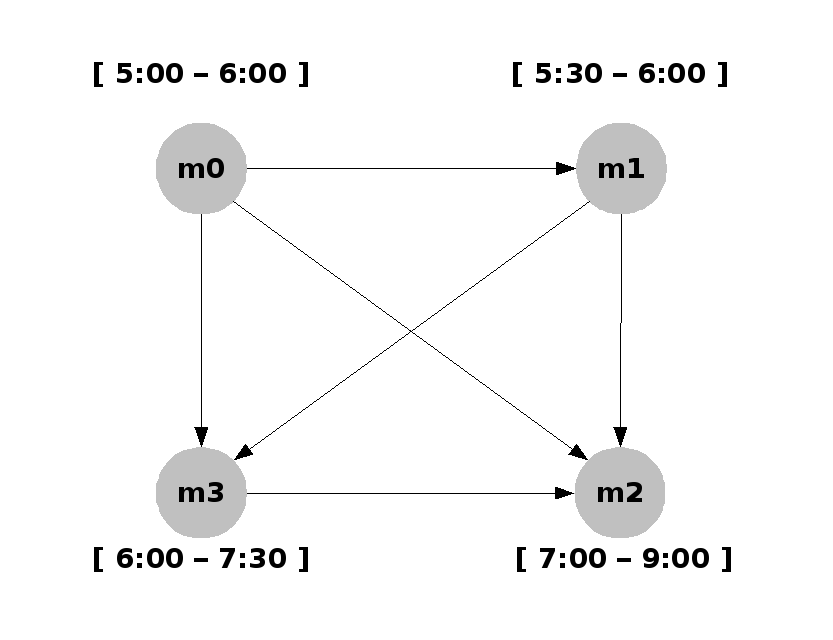
\includegraphics[width=\textwidth]{Shemas/precedence.png} \\
	\end{center}

	\end{minipage}}
	\caption{Precedence graph of the problem described in
\ref{problem_description}}
	\label{precedence}
\end{figure}

\begin{figure}[!h]
	\fbox{\begin{minipage}{0.4\textwidth}
	\begin{center}
	
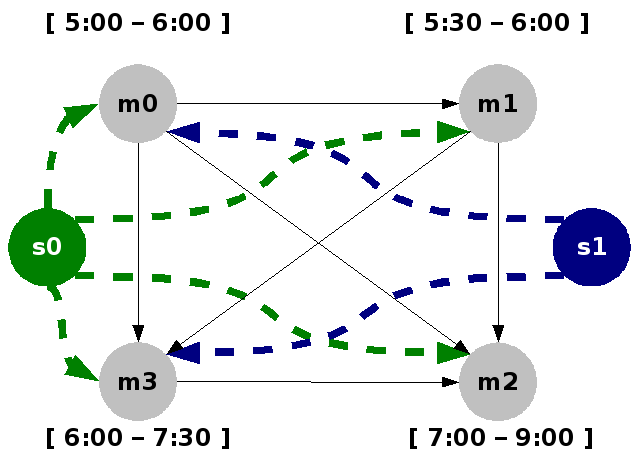
\includegraphics[width=\textwidth]{Shemas/precedence_with_vehicles.png} \\
	\end{center}

	\end{minipage}}
	\caption{The vehicles nodes are added to the precedence graph}
	\label{precedence_with_vehicles}
\end{figure}

\begin{figure}[!h]
	\fbox{\begin{minipage}{0.4\textwidth}
	\begin{center}
	
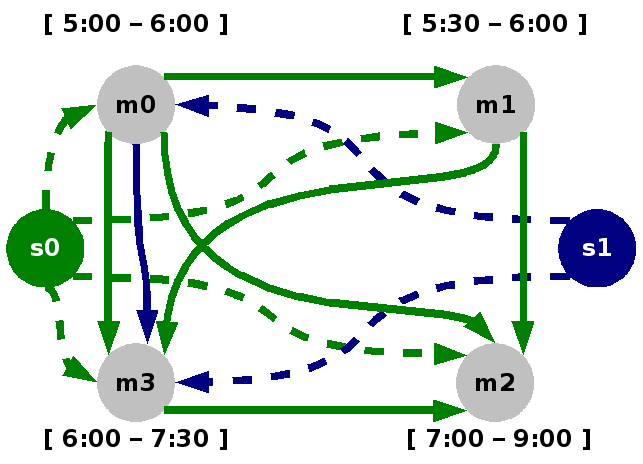
\includegraphics[width=\textwidth]{Shemas/missionGraphComplet.png} \\
		
	\end{center}

	\end{minipage}}
	\caption{Mission graph for 2 straddle carriers and 4 missions }
	\label{missiongraph}
\end{figure}



\subsubsection{Arcs weighting}

We introduce arc weights which influence the ants when moving in
the graph. The weight of an arc measures how efficient it is to assign
the two missions connected by the arc to the same carrier. This part
of our model provides flexibility and allows to test different
weighting policies.
%dire que c l'heuristique de l'algorithme

%Notre heuristique
Our policy takes into account both the cost of the mission execution and the time
windows proximity. Indeed, if two missions have time windows which are too close, and if they are assigned to the same straddle carrier, then the execution of the first mission will cause the overrunning of the time
window of the second mission. It is really important to prevent these phenomena
by modelling the linking penalty. We also define a concept of priority. The
more the end of the time window is close, the more the priority is high.
The weighting function of the arcs takes into account also the
distance between the delivery location of the first mission and the
pickup location of the second one.\\

\subsection{Colored Ant Colony Algorithm}
%$ qui explique le fonctionnement d'aco
In this algorithm, each straddle carrier has a corresponding colony of the same color. Each colony starts from the node representing its straddle carrier. Then, the ants move in the graph using only the arcs of their color. When an ant is in a node, it chooses the next node to visit according to three factors:
\begin{itemize}
 \item the pheromone rate of its own color
 \item the pheromone rate of foreign colors
 \item the weight of the arc
\end{itemize}
The ant is attracted by the pheromone of its color and repulsed by the pheromone of different colors. Once an ant have reached the chosen node, it spreads pheromone according to the quality of this choice.
When a straddle carrier of color $c$ asks for a new mission, it chooses the mission which has the highest rate of pheromone of color $c$.
The overall description of algorithm is shown on Fig. \ref{algo}.
\begin{figure}[h]
\fbox{\begin{minipage}{0.45\textwidth}
	\begin{algorithmic}[1]
		\FORALL{colony c}
			\FORALL{ant of colony c}
				\STATE choose an unvisited destination
				\STATE move towards it according to the ant speed
				\STATE spread pheromone
			\ENDFOR
		\ENDFOR
		\STATE evaporation
	\end{algorithmic}	
	
\end{minipage}}
	\caption{Colored Ant System main algorithm}
	\label{algo}
\end{figure}
	
Our ant colony approach is relevant for solving the considered problem
because of its dynamic nature, the large size of the solution space
and the real time constraint.

The main asset of ant colony is to provide an anytime solution. It is an on-line
algorithm which adapts easily to the changing environment. Indeed, ants reinforce the pheromone rates to get closer to the best solution. At the same time, evaporation process provides
a feedback control of the algorithm by preventing it to get stuck into a local
optimum and allowing dynamic events to be handled.\\

Ant colony deals with many parameters such as evaporation, solution evaluation, ants quantity and speed,
dynamic events, \textit{etc}... Here is the major weakness of this metaheuristic. Solution quality strongly depends on these interdependent settings. %Tell how difficult it is to optimize these damn parameters before running several runs !
We have tried to make these parameters self-adaptive. We use a local method to adapt some of these parameters on-line.

\subsection{Division of labor}
As there are several distinct colonies and each ant has only a local vision of its environment, there
is no way to use a pheromone spreading process based on a global characteristic.
In fact, in this architecture, a colony cannot compare the quality of its own
solution to the solutions of the other colonies. So, we must use the same
pheromone spreading process for each colony. However, we are able to adapt the
quantity of pheromone spread by ants of a colony according to the corresponding
vehicle skill for a task. Indeed, we observed that we can reduce the
serving time of mission by specializing the vehicles into a kind of missions.

We can increase the quantity of pheromone spread by
a given vehicle for tasks concerning a specific area in the
container terminal and decrease the quantity spread for the tasks located into
the other areas. At the same time, we do the opposite for all other vehicles. In this way, we try to specialize the vehicle in a kind of
tasks and we are able to regulate these quantities by taking into account both
the preference and the distance criteria.\\

This regulation keeps the benefit of allowing a vehicle to take a
mission for which it is not specialized. It is really important in some cases
where the number of missions is high because this regulation prevents the system
from having unused vehicles in an area of the terminal and unaffected missions,
close of the end of their time window, in an other area.\\

This original approach has a limit. In fact, the time needed by the adaptive
system for affecting a vehicle to a mission which does not belong to its
specialization may be considerable. For this reason, the system may become less
responsive than with no specialization.

\subsection{Reducing resources}
%How does it works
Always in a cost lowering purpose, we try to decrease the number of straddle
carriers in the system. Our current solution to the entire problem tends to
distribute the missions upon all the vehicles. So, every vehicle has almost the
same activity rate. But if this rate is under a defined lower threshold, it is possible
to conclude that a vehicle could be removed. Otherwise, if the rate is greater
than the upper threshold, it is possible to say that a new vehicle should be added to the
fleet.\\

%How to compute the target rate
The thresholds must be computed by taking into account several facts. First, it
has to deal with the quality of service. Indeed, the system must answer the
requests before the end of their time windows. Furthermore, if a vehicle is ready
to serve several missions before the beginning of their time windows, it means
that this vehicle is maybe superfluous, and the thresholds must be
modified accordingly. On the other hand, the target rate has to deal with other criteria like
the covered distance of a vehicle per mission or the ratio between the number of
vehicles and the number of missions, and it has to set these criteria against
the penalties of transcended time windows. Measuring the time of inactivity of
every straddle carrier may also lead the optimization. Concerning this last
criterion, we must interrelate the time of inactivity with the penalties of
transcended time windows.\\

%And what about dynamicity on resources
So, as for the missions arrivals into the system, the number of vehicles is
subject to dynamicity. A vehicle can break down and then must be sent to the
maintenance. In function of the failure seriousness, we can estimate the time
needed to repair the vehicle and so make it available for routing. We take a
rate of fault into account for optimizing the number of vehicles into the system
because if this number is as low as possible without transcending some time
windows, it will become too low if one vehicle of the fleet breaks down.

\section{Simulator}
%Introduction: 2 parts
The simulator has two main parts. The first one is the terminal simulation (see
Fig. \ref{tview}), and the second one is the Colored Ant Colony Optimization
System (see Fig. \ref{acoview}).
%% 1st part
The first part contains an implementation of the terminal structure and
components. Roads and crossroads provide the network of the terminal on which
straddle carriers will be able to go. Some of these roads may contain
containers. Quay crane locations are represented by these specials roads, as well as
the trucks handling locations. This terminal is built at the very beginning of
the simulation. A scenario file is read to set the terminal configuration.
%% 2nd part
The second part of the simulator contains the algorithmic view of the
simulation, \textit{i.e.} the dynamic mission graph. In this way, it shows how
the missions are chosen by the vehicles. This part of the simulator uses
GraphStream\footnote{http://graphstream-project.org/} toolkit which allows to
handle dynamic graphs easily \cite{Dutot2007}.\\

% Discrete motor and dynamicity
The simulator uses a discrete time engine which has to iterate every object of the
simulation on every time step. During the simulation, the scenario file is
read and some dynamic events are sent back to both terminal and Ant Colony
views. In this way, the system can simulate the dynamicity %??? Can I say so ?
of the incoming missions and of the vehicles availability.\\

%% Measure of dynamicity
In order to have relevant tests and results, we have to define several levels of
dynamicity. In \cite{larsen00}, Allan Larsen points out two main ways to measure the degree of dynamicity.\\

%%%dod
First, the degree of dynamism ($dod$) \cite{Lund96} is the ratio between
the number of dynamical requests and the total number of requests. The main weakness of this
measure is that it does not take  into account the arrival time of these
requests into the system. Indeed, with $dod$ if the requests come into the
system at the beginning of the day, the system is as dynamic as if they come
late in the day. Yet, the later these requests are known, the shorter is the
delivery delay. This lateness impacts on the performance of the system.\\

%%%edod
For this reason, Larsen \textit{et al.} in \cite{larsen00} defined the effective degree
of dynamism ($edod$) by the following formula: \\
\begin{equation}
	edod\;=\; \frac{\sum_{i=1}^{\eta_d}\frac{t_i}{T}}{\eta_d+\eta_s}
	%\label{edod}
\end{equation}
Here, $\eta_s$ and $\eta_d$ are respectively the number of static and dynamic
requests, $t_i$ is the arrival time of request $i$ (with $0 < t_i < T $) and $T$ is the time of
the simulation end. This measure takes into account the average of the incoming
time of the requests into the system. The more the dynamical requests come late,
the more $edod$ will be high. If $edod=0$, then the system is totally static.
Else, if $edod = 1$, then the system is purely dynamic.


% Mission scheduling
Every straddle carrier on the terminal simulation receives a schedule from the
Colored Ant Colony System. Then they act in function of it and move to their
pick-up location. Once they have picked-up their container, they move to the
delivery location to achieve their mission. At the same time, the mission graph
is dynamically updated and the colored ants keep colonizing it.\\

\begin{figure}
\fbox{\begin{minipage}{0.45\textwidth}
	\begin{center}
		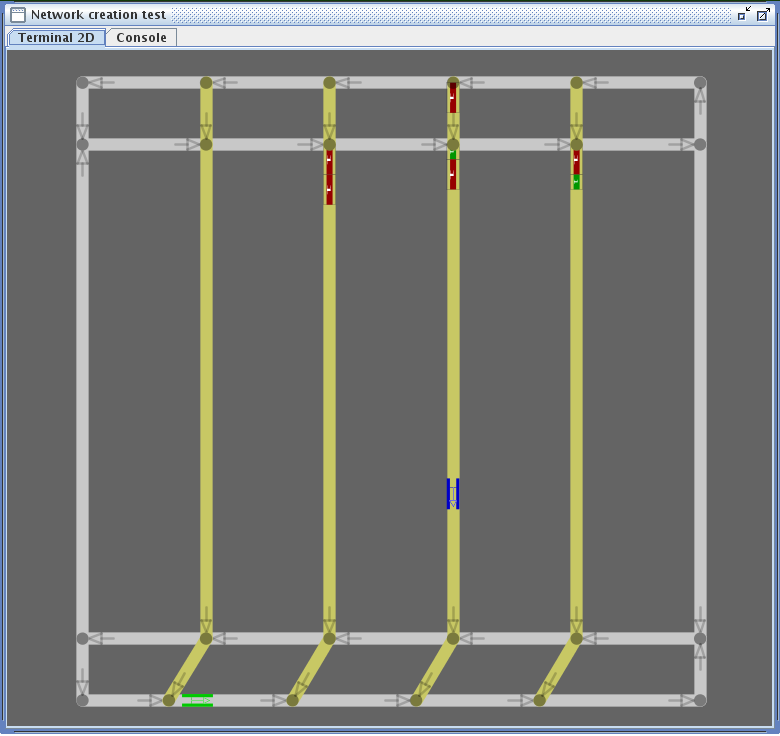
\includegraphics[width=\textwidth]{Shemas/terminal.png}
	\end{center}
\end{minipage}}
\caption{Terminal view in the simulator}
\label{tview}
\end{figure}

Simulator gives information about each mission like its length, container,
straddle carrier, pickup and delivery time windows, \textit{etc.} and about other parts of the terminal like the state of the roads for instance.

\begin{figure*}
\fbox{\begin{minipage}{\textwidth}
 	\begin{center}
	
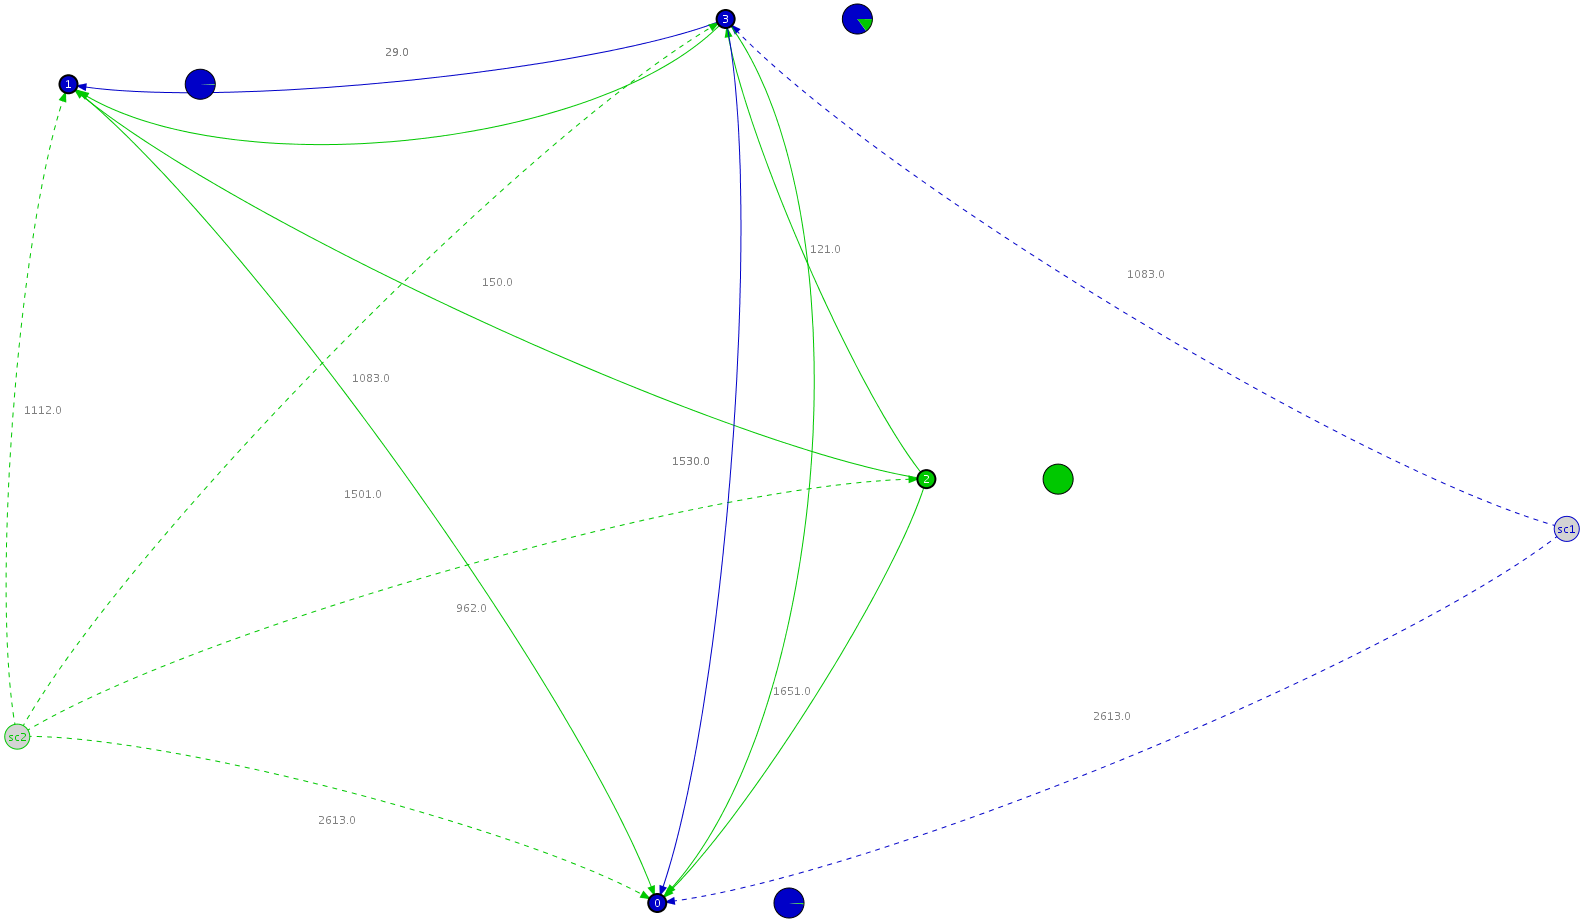
\includegraphics[width=0.9\textwidth]{Shemas/fourMissionsTwoVehicles.png}
	\end{center}
\end{minipage}}
	\caption{Mission graph view in the simulator}
	\label{acoview}
\end{figure*}

\section{Preliminary Results}
%description des tests
As we are still collecting real data from our partners, we are just able to test the relevance of our modelling and of our algorithm on simulated data. For this purpose, we have first
run a simulation with a static context, which means that every mission is known at the very beginning of the simulation and that the resources are always
available. In a second time, we have added dynamic events such as new incoming missions. For each simulation we have measured the global time
needed for achieving all the missions, the number of overrun time windows and the global overrun time. %CHECK FOR OVERRUN !!!
We consider that a time window has been overrun if the non respect of this time window represents a penalty for the container terminal. Indeed, if we overrun the time window of a mission in which we have to move a container from or toward a truck for instance, then the truck will ask for a compensation.


%Resultats
\begin{figure}
%\fbox{\begin{minipage}{0.45\textwidth}
 	\begin{center}
	\begin{tabular}{*{5}{|l|c|c|c}}
		\hline
						& Static& Half Dynamic & Dynamic \\
		\hline
		$dod$				& 0 	&0.5 	& 1 	 \\
		$edod$				& 0 	&0.25	& 1 	\\
		%Number of vehicles		& 3	& 3	& 3	\\
		%Number of missions		& 12	& 12	& 12	\\
		\hline
		End time 			&22693	& 22276	& 22693   \\
		\hline		
		Number of overrun tw		&3	&5 	& 7 \\
		\hline		
		Overrun time penalty		&6467	&8477	& 12485\\
		\hline
	
	\end{tabular}
	

	\end{center}
%\end{minipage}}
	\caption{Results of simulations}
	\label{results}
 
\end{figure}

%Commentaires des résultats
Figure \ref{results} shows the results of three instances containing 12 missions and 3 straddle carriers. The only difference between these instances is their degree of dynamicity. Indeed, we have only changed the arrival time of these missions into the system to make them more or less dynamic.

As we can see in Fig. \ref{results}, our algorithm seems to act as expected. It means that the more the missions are known in advance, the better is the performance. The worst case occurs when the mission is known at the very beginning of its time window. These are preliminary results and we have not tested all the parameters of the ant algorithm yet.

%Est-ce qu'on evoque le fait que le nombre de tw respectes est lineaire a dod ? Le pb c'est que c pas tt a fait lineaire a edod (qui est en fait edor pour nous (T = twP.from))...
\section{Conclusion}

The problem considered in this paper belongs to the Dynamic Pickup and Delivery Problem with Time Windows class. However, it does not exactly fit. So it is an original unsolved problem. We propose to solve it using swarm intelligence method. An Ant Colony System is being developed. It uses colored ants and a graph modelling in order to plan a schedule. Moreover, we are trying to minimize the number of vehicles into the fleet in order to both maintain a sufficient quality of service and reduce costs. A simulator able to reproduce the behavior of such a system and to handle dynamic events is being developed. The preliminary results confirm that our algorithm is able to handle dynamicity and we are actually collecting data in order to compare the performance of our system into a container terminal environment with the current scheduling methods used in a terminal of the seaport of Le Havre in France.
		
\bibliographystyle{IEEEtran}
\bibliography{IEEEabrv,biblio}

% that's all folks
\end{document}
